% SOURCE: edit-harness/results/frame_a/cells/cell_*_real_MIX_B_*.json
% !TEX encoding = UTF-8 Unicode
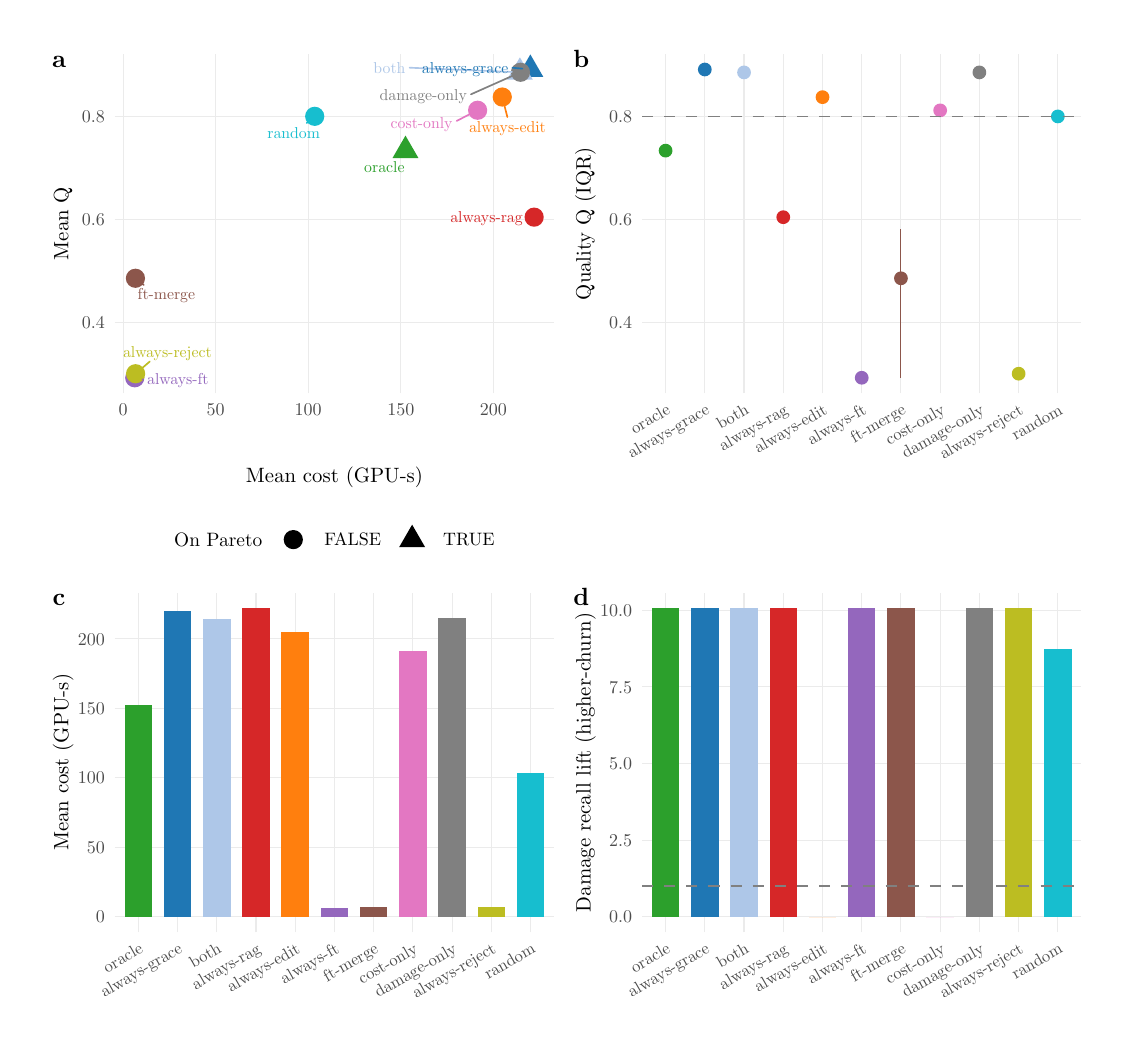
\begin{tikzpicture}[x=1pt,y=1pt]
\definecolor{fillColor}{RGB}{255,255,255}
\path[use as bounding box,fill=fillColor,fill opacity=0.00] (0,0) rectangle (390.26,361.35);
\begin{scope}
\path[clip] (  0.00,  0.00) rectangle (390.26,361.35);
\definecolor{drawColor}{RGB}{255,255,255}
\definecolor{fillColor}{RGB}{255,255,255}

\path[draw=drawColor,line width= 0.6pt,line join=round,line cap=round,fill=fillColor] (  0.00,  0.00) rectangle (390.26,361.35);
\end{scope}
\begin{scope}
\path[clip] (  5.50,161.14) rectangle (194.23,355.85);
\definecolor{fillColor}{RGB}{255,255,255}

\path[fill=fillColor] (  5.50,161.14) rectangle (194.23,355.85);
\end{scope}
\begin{scope}
\path[clip] (194.23,161.14) rectangle (384.76,355.85);
\definecolor{fillColor}{RGB}{255,255,255}

\path[fill=fillColor] (194.23,161.14) rectangle (384.76,355.85);
\end{scope}
\begin{scope}
\path[clip] (  5.50,  5.50) rectangle (194.23,161.14);
\definecolor{fillColor}{RGB}{255,255,255}

\path[fill=fillColor] (  5.50,  5.50) rectangle (194.23,161.14);
\end{scope}
\begin{scope}
\path[clip] (194.23,  5.50) rectangle (384.76,161.14);
\definecolor{fillColor}{RGB}{255,255,255}

\path[fill=fillColor] (194.23,  5.50) rectangle (384.76,161.14);
\end{scope}
\begin{scope}
\path[clip] ( 31.47,229.26) rectangle (190.23,351.85);
\definecolor{drawColor}{gray}{0.92}

\path[draw=drawColor,line width= 0.4pt,line join=round] ( 31.47,254.91) --
	(190.23,254.91);

\path[draw=drawColor,line width= 0.4pt,line join=round] ( 31.47,292.13) --
	(190.23,292.13);

\path[draw=drawColor,line width= 0.4pt,line join=round] ( 31.47,329.36) --
	(190.23,329.36);

\path[draw=drawColor,line width= 0.4pt,line join=round] ( 34.50,229.26) --
	( 34.50,351.85);

\path[draw=drawColor,line width= 0.4pt,line join=round] ( 67.94,229.26) --
	( 67.94,351.85);

\path[draw=drawColor,line width= 0.4pt,line join=round] (101.38,229.26) --
	(101.38,351.85);

\path[draw=drawColor,line width= 0.4pt,line join=round] (134.82,229.26) --
	(134.82,351.85);

\path[draw=drawColor,line width= 0.4pt,line join=round] (168.26,229.26) --
	(168.26,351.85);
\definecolor{fillColor}{RGB}{44,160,44}

\path[fill=fillColor] (136.52,322.35) --
	(141.19,314.25) --
	(131.84,314.25) --
	cycle;
\definecolor{fillColor}{RGB}{31,119,180}

\path[fill=fillColor] (181.64,351.68) --
	(186.31,343.58) --
	(176.96,343.58) --
	cycle;
\definecolor{fillColor}{RGB}{174,199,232}

\path[fill=fillColor] (177.86,350.63) --
	(182.54,342.53) --
	(173.19,342.53) --
	cycle;
\definecolor{fillColor}{RGB}{214,39,40}

\path[fill=fillColor] (183.01,292.88) circle (  3.47);
\definecolor{fillColor}{RGB}{255,127,14}

\path[fill=fillColor] (171.50,336.28) circle (  3.47);
\definecolor{fillColor}{RGB}{148,103,189}

\path[fill=fillColor] ( 38.69,234.83) circle (  3.47);
\definecolor{fillColor}{RGB}{140,86,75}

\path[fill=fillColor] ( 38.94,270.79) circle (  3.47);
\definecolor{fillColor}{RGB}{227,119,194}

\path[fill=fillColor] (162.58,331.50) circle (  3.47);
\definecolor{fillColor}{gray}{0.50}

\path[fill=fillColor] (178.07,345.23) circle (  3.47);
\definecolor{fillColor}{RGB}{188,189,34}

\path[fill=fillColor] ( 39.00,236.30) circle (  3.47);
\definecolor{fillColor}{RGB}{23,190,207}

\path[fill=fillColor] (103.72,329.31) circle (  3.47);
\definecolor{drawColor}{RGB}{44,160,44}

\path[draw=drawColor,line width= 0.6pt,line join=round,line cap=round] (133.63,314.53) -- (134.31,315.10);
\definecolor{drawColor}{RGB}{31,119,180}

\path[draw=drawColor,line width= 0.6pt,line join=round,line cap=round] (175.17,346.87) -- (178.77,346.54);
\definecolor{drawColor}{RGB}{174,199,232}

\path[draw=drawColor,line width= 0.6pt,line join=round,line cap=round] (138.00,346.88) -- (174.99,345.35);
\definecolor{drawColor}{RGB}{255,127,14}

\path[draw=drawColor,line width= 0.6pt,line join=round,line cap=round] (173.33,329.06) -- (172.21,333.49);
\definecolor{drawColor}{RGB}{148,103,189}

\path[draw=drawColor,line width= 0.6pt,line join=round,line cap=round] ( 41.68,234.25) -- ( 41.51,234.28);
\definecolor{drawColor}{RGB}{140,86,75}

\path[draw=drawColor,line width= 0.6pt,line join=round,line cap=round] ( 41.95,268.38) -- ( 41.19,268.99);
\definecolor{drawColor}{RGB}{227,119,194}

\path[draw=drawColor,line width= 0.6pt,line join=round,line cap=round] (155.02,327.66) -- (160.02,330.20);
\definecolor{drawColor}{gray}{0.50}

\path[draw=drawColor,line width= 0.6pt,line join=round,line cap=round] (160.17,337.26) -- (175.44,344.06);
\definecolor{drawColor}{RGB}{188,189,34}

\path[draw=drawColor,line width= 0.6pt,line join=round,line cap=round] ( 44.11,240.70) -- ( 41.18,238.18);
\definecolor{drawColor}{RGB}{23,190,207}

\path[draw=drawColor,line width= 0.6pt,line join=round,line cap=round] (100.84,326.90) -- (101.51,327.47);
\definecolor{drawColor}{RGB}{44,160,44}

\node[text=drawColor,anchor=base,inner sep=0pt, outer sep=0pt, scale=  0.57] at (128.90,309.11) {oracle};
\definecolor{drawColor}{RGB}{31,119,180}

\node[text=drawColor,anchor=base,inner sep=0pt, outer sep=0pt, scale=  0.57] at (158.07,344.92) {always-grace};
\definecolor{drawColor}{RGB}{174,199,232}

\node[text=drawColor,anchor=base,inner sep=0pt, outer sep=0pt, scale=  0.57] at (130.72,344.92) {both};
\definecolor{drawColor}{RGB}{214,39,40}

\node[text=drawColor,anchor=base,inner sep=0pt, outer sep=0pt, scale=  0.57] at (165.81,290.79) {always-rag};
\definecolor{drawColor}{RGB}{255,127,14}

\node[text=drawColor,anchor=base,inner sep=0pt, outer sep=0pt, scale=  0.57] at (173.37,323.63) {always-edit};
\definecolor{drawColor}{RGB}{148,103,189}

\node[text=drawColor,anchor=base,inner sep=0pt, outer sep=0pt, scale=  0.57] at ( 54.27,232.27) {always-ft};
\definecolor{drawColor}{RGB}{140,86,75}

\node[text=drawColor,anchor=base,inner sep=0pt, outer sep=0pt, scale=  0.57] at ( 50.13,262.95) {ft-merge};
\definecolor{drawColor}{RGB}{227,119,194}

\node[text=drawColor,anchor=base,inner sep=0pt, outer sep=0pt, scale=  0.57] at (142.36,325.02) {cost-only};
\definecolor{drawColor}{gray}{0.50}

\node[text=drawColor,anchor=base,inner sep=0pt, outer sep=0pt, scale=  0.57] at (142.94,334.98) {damage-only};
\definecolor{drawColor}{RGB}{188,189,34}

\node[text=drawColor,anchor=base,inner sep=0pt, outer sep=0pt, scale=  0.57] at ( 50.47,242.20) {always-reject};
\definecolor{drawColor}{RGB}{23,190,207}

\node[text=drawColor,anchor=base,inner sep=0pt, outer sep=0pt, scale=  0.57] at ( 96.11,321.48) {random};
\end{scope}
\begin{scope}
\path[clip] (  0.00,  0.00) rectangle (390.26,361.35);
\definecolor{drawColor}{gray}{0.30}

\node[text=drawColor,anchor=base east,inner sep=0pt, outer sep=0pt, scale=  0.65] at ( 27.87,252.67) {0.4};

\node[text=drawColor,anchor=base east,inner sep=0pt, outer sep=0pt, scale=  0.65] at ( 27.87,289.89) {0.6};

\node[text=drawColor,anchor=base east,inner sep=0pt, outer sep=0pt, scale=  0.65] at ( 27.87,327.12) {0.8};
\end{scope}
\begin{scope}
\path[clip] (  0.00,  0.00) rectangle (390.26,361.35);
\definecolor{drawColor}{gray}{0.30}

\node[text=drawColor,anchor=base,inner sep=0pt, outer sep=0pt, scale=  0.65] at ( 34.50,221.18) {0};

\node[text=drawColor,anchor=base,inner sep=0pt, outer sep=0pt, scale=  0.65] at ( 67.94,221.18) {50};

\node[text=drawColor,anchor=base,inner sep=0pt, outer sep=0pt, scale=  0.65] at (101.38,221.18) {100};

\node[text=drawColor,anchor=base,inner sep=0pt, outer sep=0pt, scale=  0.65] at (134.82,221.18) {150};

\node[text=drawColor,anchor=base,inner sep=0pt, outer sep=0pt, scale=  0.65] at (168.26,221.18) {200};
\end{scope}
\begin{scope}
\path[clip] (  0.00,  0.00) rectangle (390.26,361.35);
\definecolor{drawColor}{RGB}{0,0,0}

\node[text=drawColor,anchor=base,inner sep=0pt, outer sep=0pt, scale=  0.75] at (110.85,197.05) {Mean cost (GPU-s)};
\end{scope}
\begin{scope}
\path[clip] (  0.00,  0.00) rectangle (390.26,361.35);
\definecolor{drawColor}{RGB}{0,0,0}

\node[text=drawColor,rotate= 90.00,anchor=base,inner sep=0pt, outer sep=0pt, scale=  0.75] at ( 14.67,290.55) {Mean Q};
\end{scope}
\begin{scope}
\path[clip] (  0.00,  0.00) rectangle (390.26,361.35);
\definecolor{drawColor}{RGB}{0,0,0}

\node[text=drawColor,anchor=base west,inner sep=0pt, outer sep=0pt, scale=  0.70] at ( 52.95,173.95) {On Pareto};
\end{scope}
\begin{scope}
\path[clip] (  0.00,  0.00) rectangle (390.26,361.35);
\definecolor{fillColor}{RGB}{0,0,0}

\path[fill=fillColor] ( 95.98,176.36) circle (  3.47);
\end{scope}
\begin{scope}
\path[clip] (  0.00,  0.00) rectangle (390.26,361.35);
\definecolor{fillColor}{RGB}{0,0,0}

\path[fill=fillColor] (138.92,181.76) --
	(143.60,173.66) --
	(134.25,173.66) --
	cycle;
\end{scope}
\begin{scope}
\path[clip] (  0.00,  0.00) rectangle (390.26,361.35);
\definecolor{drawColor}{RGB}{0,0,0}

\node[text=drawColor,anchor=base west,inner sep=0pt, outer sep=0pt, scale=  0.65] at (107.21,174.12) {FALSE};
\end{scope}
\begin{scope}
\path[clip] (  0.00,  0.00) rectangle (390.26,361.35);
\definecolor{drawColor}{RGB}{0,0,0}

\node[text=drawColor,anchor=base west,inner sep=0pt, outer sep=0pt, scale=  0.65] at (150.15,174.12) {TRUE};
\end{scope}
\begin{scope}
\path[clip] (  0.00,  0.00) rectangle (390.26,361.35);
\definecolor{drawColor}{RGB}{0,0,0}

\node[text=drawColor,anchor=base,inner sep=0pt, outer sep=0pt, scale=  0.90] at ( 11.31,346.88) {\bfseries a};
\end{scope}
\begin{scope}
\path[clip] (222.00,229.26) rectangle (380.76,351.85);
\definecolor{drawColor}{gray}{0.92}

\path[draw=drawColor,line width= 0.4pt,line join=round] (222.00,254.91) --
	(380.76,254.91);

\path[draw=drawColor,line width= 0.4pt,line join=round] (222.00,292.11) --
	(380.76,292.11);

\path[draw=drawColor,line width= 0.4pt,line join=round] (222.00,329.32) --
	(380.76,329.32);

\path[draw=drawColor,line width= 0.4pt,line join=round] (230.51,229.26) --
	(230.51,351.85);

\path[draw=drawColor,line width= 0.4pt,line join=round] (244.68,229.26) --
	(244.68,351.85);

\path[draw=drawColor,line width= 0.4pt,line join=round] (258.86,229.26) --
	(258.86,351.85);

\path[draw=drawColor,line width= 0.4pt,line join=round] (273.03,229.26) --
	(273.03,351.85);

\path[draw=drawColor,line width= 0.4pt,line join=round] (287.21,229.26) --
	(287.21,351.85);

\path[draw=drawColor,line width= 0.4pt,line join=round] (301.38,229.26) --
	(301.38,351.85);

\path[draw=drawColor,line width= 0.4pt,line join=round] (315.55,229.26) --
	(315.55,351.85);

\path[draw=drawColor,line width= 0.4pt,line join=round] (329.73,229.26) --
	(329.73,351.85);

\path[draw=drawColor,line width= 0.4pt,line join=round] (343.90,229.26) --
	(343.90,351.85);

\path[draw=drawColor,line width= 0.4pt,line join=round] (358.08,229.26) --
	(358.08,351.85);

\path[draw=drawColor,line width= 0.4pt,line join=round] (372.25,229.26) --
	(372.25,351.85);
\definecolor{drawColor}{RGB}{44,160,44}

\path[draw=drawColor,line width= 0.4pt,line join=round] (230.51,316.81) -- (230.51,317.04);
\definecolor{drawColor}{RGB}{31,119,180}

\path[draw=drawColor,line width= 0.4pt,line join=round] (244.68,346.13) -- (244.68,346.28);
\definecolor{drawColor}{RGB}{174,199,232}

\path[draw=drawColor,line width= 0.4pt,line join=round] (258.86,345.08) -- (258.86,345.26);
\definecolor{drawColor}{RGB}{214,39,40}

\path[draw=drawColor,line width= 0.4pt,line join=round] (273.03,292.78) -- (273.03,293.00);
\definecolor{drawColor}{RGB}{255,127,14}

\path[draw=drawColor,line width= 0.4pt,line join=round] (287.21,335.69) -- (287.21,336.59);
\definecolor{drawColor}{RGB}{148,103,189}

\path[draw=drawColor,line width= 0.4pt,line join=round] (301.38,234.83) -- (301.38,234.85);
\definecolor{drawColor}{RGB}{140,86,75}

\path[draw=drawColor,line width= 0.4pt,line join=round] (315.55,234.85) -- (315.55,288.75);
\definecolor{drawColor}{RGB}{227,119,194}

\path[draw=drawColor,line width= 0.4pt,line join=round] (329.73,331.01) -- (329.73,332.10);
\definecolor{drawColor}{gray}{0.50}

\path[draw=drawColor,line width= 0.4pt,line join=round] (343.90,345.08) -- (343.90,345.26);
\definecolor{drawColor}{RGB}{188,189,34}

\path[draw=drawColor,line width= 0.4pt,line join=round] (358.08,236.31) -- (358.08,236.31);
\definecolor{drawColor}{RGB}{23,190,207}

\path[draw=drawColor,line width= 0.4pt,line join=round] (372.25,328.54) -- (372.25,330.01);
\definecolor{drawColor}{RGB}{44,160,44}
\definecolor{fillColor}{RGB}{44,160,44}

\path[draw=drawColor,line width= 0.5pt,line join=round,line cap=round,fill=fillColor] (230.51,316.91) circle (  2.23);
\definecolor{drawColor}{RGB}{31,119,180}
\definecolor{fillColor}{RGB}{31,119,180}

\path[draw=drawColor,line width= 0.5pt,line join=round,line cap=round,fill=fillColor] (244.68,346.23) circle (  2.23);
\definecolor{drawColor}{RGB}{174,199,232}
\definecolor{fillColor}{RGB}{174,199,232}

\path[draw=drawColor,line width= 0.5pt,line join=round,line cap=round,fill=fillColor] (258.86,345.18) circle (  2.23);
\definecolor{drawColor}{RGB}{214,39,40}
\definecolor{fillColor}{RGB}{214,39,40}

\path[draw=drawColor,line width= 0.5pt,line join=round,line cap=round,fill=fillColor] (273.03,292.86) circle (  2.23);
\definecolor{drawColor}{RGB}{255,127,14}
\definecolor{fillColor}{RGB}{255,127,14}

\path[draw=drawColor,line width= 0.5pt,line join=round,line cap=round,fill=fillColor] (287.21,336.24) circle (  2.23);
\definecolor{drawColor}{RGB}{148,103,189}
\definecolor{fillColor}{RGB}{148,103,189}

\path[draw=drawColor,line width= 0.5pt,line join=round,line cap=round,fill=fillColor] (301.38,234.84) circle (  2.23);
\definecolor{drawColor}{RGB}{140,86,75}
\definecolor{fillColor}{RGB}{140,86,75}

\path[draw=drawColor,line width= 0.5pt,line join=round,line cap=round,fill=fillColor] (315.55,270.78) circle (  2.23);
\definecolor{drawColor}{RGB}{227,119,194}
\definecolor{fillColor}{RGB}{227,119,194}

\path[draw=drawColor,line width= 0.5pt,line join=round,line cap=round,fill=fillColor] (329.73,331.46) circle (  2.23);
\definecolor{drawColor}{gray}{0.50}
\definecolor{fillColor}{gray}{0.50}

\path[draw=drawColor,line width= 0.5pt,line join=round,line cap=round,fill=fillColor] (343.90,345.18) circle (  2.23);
\definecolor{drawColor}{RGB}{188,189,34}
\definecolor{fillColor}{RGB}{188,189,34}

\path[draw=drawColor,line width= 0.5pt,line join=round,line cap=round,fill=fillColor] (358.08,236.31) circle (  2.23);
\definecolor{drawColor}{RGB}{23,190,207}
\definecolor{fillColor}{RGB}{23,190,207}

\path[draw=drawColor,line width= 0.5pt,line join=round,line cap=round,fill=fillColor] (372.25,329.27) circle (  2.23);
\definecolor{drawColor}{gray}{0.50}

\path[draw=drawColor,line width= 0.5pt,dash pattern=on 4pt off 4pt ,line join=round] (222.00,329.27) -- (380.76,329.27);
\end{scope}
\begin{scope}
\path[clip] (  0.00,  0.00) rectangle (390.26,361.35);
\definecolor{drawColor}{gray}{0.30}

\node[text=drawColor,anchor=base east,inner sep=0pt, outer sep=0pt, scale=  0.65] at (218.40,252.67) {0.4};

\node[text=drawColor,anchor=base east,inner sep=0pt, outer sep=0pt, scale=  0.65] at (218.40,289.87) {0.6};

\node[text=drawColor,anchor=base east,inner sep=0pt, outer sep=0pt, scale=  0.65] at (218.40,327.08) {0.8};
\end{scope}
\begin{scope}
\path[clip] (  0.00,  0.00) rectangle (390.26,361.35);
\definecolor{drawColor}{gray}{0.30}

\node[text=drawColor,rotate= 30.00,anchor=base east,inner sep=0pt, outer sep=0pt, scale=  0.60] at (232.57,222.08) {oracle};

\node[text=drawColor,rotate= 30.00,anchor=base east,inner sep=0pt, outer sep=0pt, scale=  0.60] at (246.75,222.08) {always-grace};

\node[text=drawColor,rotate= 30.00,anchor=base east,inner sep=0pt, outer sep=0pt, scale=  0.60] at (260.92,222.08) {both};

\node[text=drawColor,rotate= 30.00,anchor=base east,inner sep=0pt, outer sep=0pt, scale=  0.60] at (275.10,222.08) {always-rag};

\node[text=drawColor,rotate= 30.00,anchor=base east,inner sep=0pt, outer sep=0pt, scale=  0.60] at (289.27,222.08) {always-edit};

\node[text=drawColor,rotate= 30.00,anchor=base east,inner sep=0pt, outer sep=0pt, scale=  0.60] at (303.45,222.08) {always-ft};

\node[text=drawColor,rotate= 30.00,anchor=base east,inner sep=0pt, outer sep=0pt, scale=  0.60] at (317.62,222.08) {ft-merge};

\node[text=drawColor,rotate= 30.00,anchor=base east,inner sep=0pt, outer sep=0pt, scale=  0.60] at (331.80,222.08) {cost-only};

\node[text=drawColor,rotate= 30.00,anchor=base east,inner sep=0pt, outer sep=0pt, scale=  0.60] at (345.97,222.08) {damage-only};

\node[text=drawColor,rotate= 30.00,anchor=base east,inner sep=0pt, outer sep=0pt, scale=  0.60] at (360.14,222.08) {always-reject};

\node[text=drawColor,rotate= 30.00,anchor=base east,inner sep=0pt, outer sep=0pt, scale=  0.60] at (374.32,222.08) {random};
\end{scope}
\begin{scope}
\path[clip] (  0.00,  0.00) rectangle (390.26,361.35);
\definecolor{drawColor}{RGB}{0,0,0}

\node[text=drawColor,rotate= 90.00,anchor=base,inner sep=0pt, outer sep=0pt, scale=  0.75] at (203.39,290.55) {Quality Q (IQR)};
\end{scope}
\begin{scope}
\path[clip] (  0.00,  0.00) rectangle (390.26,361.35);
\definecolor{drawColor}{RGB}{0,0,0}

\node[text=drawColor,anchor=base,inner sep=0pt, outer sep=0pt, scale=  0.90] at (200.05,346.88) {\bfseries b};
\end{scope}
\begin{scope}
\path[clip] ( 31.47, 34.54) rectangle (190.23,157.14);
\definecolor{drawColor}{gray}{0.92}

\path[draw=drawColor,line width= 0.4pt,line join=round] ( 31.47, 40.12) --
	(190.23, 40.12);

\path[draw=drawColor,line width= 0.4pt,line join=round] ( 31.47, 65.21) --
	(190.23, 65.21);

\path[draw=drawColor,line width= 0.4pt,line join=round] ( 31.47, 90.30) --
	(190.23, 90.30);

\path[draw=drawColor,line width= 0.4pt,line join=round] ( 31.47,115.40) --
	(190.23,115.40);

\path[draw=drawColor,line width= 0.4pt,line join=round] ( 31.47,140.49) --
	(190.23,140.49);

\path[draw=drawColor,line width= 0.4pt,line join=round] ( 39.98, 34.54) --
	( 39.98,157.14);

\path[draw=drawColor,line width= 0.4pt,line join=round] ( 54.15, 34.54) --
	( 54.15,157.14);

\path[draw=drawColor,line width= 0.4pt,line join=round] ( 68.32, 34.54) --
	( 68.32,157.14);

\path[draw=drawColor,line width= 0.4pt,line join=round] ( 82.50, 34.54) --
	( 82.50,157.14);

\path[draw=drawColor,line width= 0.4pt,line join=round] ( 96.67, 34.54) --
	( 96.67,157.14);

\path[draw=drawColor,line width= 0.4pt,line join=round] (110.85, 34.54) --
	(110.85,157.14);

\path[draw=drawColor,line width= 0.4pt,line join=round] (125.02, 34.54) --
	(125.02,157.14);

\path[draw=drawColor,line width= 0.4pt,line join=round] (139.20, 34.54) --
	(139.20,157.14);

\path[draw=drawColor,line width= 0.4pt,line join=round] (153.37, 34.54) --
	(153.37,157.14);

\path[draw=drawColor,line width= 0.4pt,line join=round] (167.55, 34.54) --
	(167.55,157.14);

\path[draw=drawColor,line width= 0.4pt,line join=round] (181.72, 34.54) --
	(181.72,157.14);
\definecolor{fillColor}{RGB}{44,160,44}

\path[fill=fillColor] ( 35.01, 40.12) rectangle ( 44.94,116.67);
\definecolor{fillColor}{RGB}{31,119,180}

\path[fill=fillColor] ( 49.19, 40.12) rectangle ( 59.11,150.53);
\definecolor{fillColor}{RGB}{174,199,232}

\path[fill=fillColor] ( 63.36, 40.12) rectangle ( 73.29,147.70);
\definecolor{fillColor}{RGB}{214,39,40}

\path[fill=fillColor] ( 77.54, 40.12) rectangle ( 87.46,151.56);
\definecolor{fillColor}{RGB}{255,127,14}

\path[fill=fillColor] ( 91.71, 40.12) rectangle (101.64,142.93);
\definecolor{fillColor}{RGB}{148,103,189}

\path[fill=fillColor] (105.89, 40.12) rectangle (115.81, 43.26);
\definecolor{fillColor}{RGB}{140,86,75}

\path[fill=fillColor] (120.06, 40.12) rectangle (129.98, 43.45);
\definecolor{fillColor}{RGB}{227,119,194}

\path[fill=fillColor] (134.24, 40.12) rectangle (144.16,136.23);
\definecolor{fillColor}{gray}{0.50}

\path[fill=fillColor] (148.41, 40.12) rectangle (158.33,147.86);
\definecolor{fillColor}{RGB}{188,189,34}

\path[fill=fillColor] (162.59, 40.12) rectangle (172.51, 43.49);
\definecolor{fillColor}{RGB}{23,190,207}

\path[fill=fillColor] (176.76, 40.12) rectangle (186.68, 92.06);
\end{scope}
\begin{scope}
\path[clip] (  0.00,  0.00) rectangle (390.26,361.35);
\definecolor{drawColor}{gray}{0.30}

\node[text=drawColor,anchor=base east,inner sep=0pt, outer sep=0pt, scale=  0.65] at ( 27.87, 37.88) {0};

\node[text=drawColor,anchor=base east,inner sep=0pt, outer sep=0pt, scale=  0.65] at ( 27.87, 62.97) {50};

\node[text=drawColor,anchor=base east,inner sep=0pt, outer sep=0pt, scale=  0.65] at ( 27.87, 88.07) {100};

\node[text=drawColor,anchor=base east,inner sep=0pt, outer sep=0pt, scale=  0.65] at ( 27.87,113.16) {150};

\node[text=drawColor,anchor=base east,inner sep=0pt, outer sep=0pt, scale=  0.65] at ( 27.87,138.25) {200};
\end{scope}
\begin{scope}
\path[clip] (  0.00,  0.00) rectangle (390.26,361.35);
\definecolor{drawColor}{gray}{0.30}

\node[text=drawColor,rotate= 30.00,anchor=base east,inner sep=0pt, outer sep=0pt, scale=  0.60] at ( 42.04, 27.36) {oracle};

\node[text=drawColor,rotate= 30.00,anchor=base east,inner sep=0pt, outer sep=0pt, scale=  0.60] at ( 56.22, 27.36) {always-grace};

\node[text=drawColor,rotate= 30.00,anchor=base east,inner sep=0pt, outer sep=0pt, scale=  0.60] at ( 70.39, 27.36) {both};

\node[text=drawColor,rotate= 30.00,anchor=base east,inner sep=0pt, outer sep=0pt, scale=  0.60] at ( 84.57, 27.36) {always-rag};

\node[text=drawColor,rotate= 30.00,anchor=base east,inner sep=0pt, outer sep=0pt, scale=  0.60] at ( 98.74, 27.36) {always-edit};

\node[text=drawColor,rotate= 30.00,anchor=base east,inner sep=0pt, outer sep=0pt, scale=  0.60] at (112.91, 27.36) {always-ft};

\node[text=drawColor,rotate= 30.00,anchor=base east,inner sep=0pt, outer sep=0pt, scale=  0.60] at (127.09, 27.36) {ft-merge};

\node[text=drawColor,rotate= 30.00,anchor=base east,inner sep=0pt, outer sep=0pt, scale=  0.60] at (141.26, 27.36) {cost-only};

\node[text=drawColor,rotate= 30.00,anchor=base east,inner sep=0pt, outer sep=0pt, scale=  0.60] at (155.44, 27.36) {damage-only};

\node[text=drawColor,rotate= 30.00,anchor=base east,inner sep=0pt, outer sep=0pt, scale=  0.60] at (169.61, 27.36) {always-reject};

\node[text=drawColor,rotate= 30.00,anchor=base east,inner sep=0pt, outer sep=0pt, scale=  0.60] at (183.79, 27.36) {random};
\end{scope}
\begin{scope}
\path[clip] (  0.00,  0.00) rectangle (390.26,361.35);
\definecolor{drawColor}{RGB}{0,0,0}

\node[text=drawColor,rotate= 90.00,anchor=base,inner sep=0pt, outer sep=0pt, scale=  0.75] at ( 14.67, 95.84) {Mean cost (GPU-s)};
\end{scope}
\begin{scope}
\path[clip] (  0.00,  0.00) rectangle (390.26,361.35);
\definecolor{drawColor}{RGB}{0,0,0}

\node[text=drawColor,anchor=base,inner sep=0pt, outer sep=0pt, scale=  0.90] at ( 11.31,152.55) {\bfseries c};
\end{scope}
\begin{scope}
\path[clip] (222.00, 34.54) rectangle (380.76,157.14);
\definecolor{drawColor}{gray}{0.92}

\path[draw=drawColor,line width= 0.4pt,line join=round] (222.00, 40.12) --
	(380.76, 40.12);

\path[draw=drawColor,line width= 0.4pt,line join=round] (222.00, 67.78) --
	(380.76, 67.78);

\path[draw=drawColor,line width= 0.4pt,line join=round] (222.00, 95.45) --
	(380.76, 95.45);

\path[draw=drawColor,line width= 0.4pt,line join=round] (222.00,123.12) --
	(380.76,123.12);

\path[draw=drawColor,line width= 0.4pt,line join=round] (222.00,150.78) --
	(380.76,150.78);

\path[draw=drawColor,line width= 0.4pt,line join=round] (230.51, 34.54) --
	(230.51,157.14);

\path[draw=drawColor,line width= 0.4pt,line join=round] (244.68, 34.54) --
	(244.68,157.14);

\path[draw=drawColor,line width= 0.4pt,line join=round] (258.86, 34.54) --
	(258.86,157.14);

\path[draw=drawColor,line width= 0.4pt,line join=round] (273.03, 34.54) --
	(273.03,157.14);

\path[draw=drawColor,line width= 0.4pt,line join=round] (287.21, 34.54) --
	(287.21,157.14);

\path[draw=drawColor,line width= 0.4pt,line join=round] (301.38, 34.54) --
	(301.38,157.14);

\path[draw=drawColor,line width= 0.4pt,line join=round] (315.55, 34.54) --
	(315.55,157.14);

\path[draw=drawColor,line width= 0.4pt,line join=round] (329.73, 34.54) --
	(329.73,157.14);

\path[draw=drawColor,line width= 0.4pt,line join=round] (343.90, 34.54) --
	(343.90,157.14);

\path[draw=drawColor,line width= 0.4pt,line join=round] (358.08, 34.54) --
	(358.08,157.14);

\path[draw=drawColor,line width= 0.4pt,line join=round] (372.25, 34.54) --
	(372.25,157.14);
\definecolor{fillColor}{RGB}{44,160,44}

\path[fill=fillColor] (225.55, 40.12) rectangle (235.47,151.56);
\definecolor{fillColor}{RGB}{31,119,180}

\path[fill=fillColor] (239.72, 40.12) rectangle (249.64,151.56);
\definecolor{fillColor}{RGB}{174,199,232}

\path[fill=fillColor] (253.90, 40.12) rectangle (263.82,151.56);
\definecolor{fillColor}{RGB}{214,39,40}

\path[fill=fillColor] (268.07, 40.12) rectangle (277.99,151.56);
\definecolor{fillColor}{RGB}{255,127,14}

\path[fill=fillColor] (282.24, 40.12) rectangle (292.17, 40.12);
\definecolor{fillColor}{RGB}{148,103,189}

\path[fill=fillColor] (296.42, 40.12) rectangle (306.34,151.56);
\definecolor{fillColor}{RGB}{140,86,75}

\path[fill=fillColor] (310.59, 40.12) rectangle (320.52,151.56);
\definecolor{fillColor}{RGB}{227,119,194}

\path[fill=fillColor] (324.77, 40.12) rectangle (334.69, 40.12);
\definecolor{fillColor}{gray}{0.50}

\path[fill=fillColor] (338.94, 40.12) rectangle (348.87,151.56);
\definecolor{fillColor}{RGB}{188,189,34}

\path[fill=fillColor] (353.12, 40.12) rectangle (363.04,151.56);
\definecolor{fillColor}{RGB}{23,190,207}

\path[fill=fillColor] (367.29, 40.12) rectangle (377.21,136.70);
\definecolor{drawColor}{gray}{0.50}

\path[draw=drawColor,line width= 0.5pt,dash pattern=on 4pt off 4pt ,line join=round] (222.00, 51.18) -- (380.76, 51.18);
\end{scope}
\begin{scope}
\path[clip] (  0.00,  0.00) rectangle (390.26,361.35);
\definecolor{drawColor}{gray}{0.30}

\node[text=drawColor,anchor=base east,inner sep=0pt, outer sep=0pt, scale=  0.65] at (218.40, 37.88) {0.0};

\node[text=drawColor,anchor=base east,inner sep=0pt, outer sep=0pt, scale=  0.65] at (218.40, 65.54) {2.5};

\node[text=drawColor,anchor=base east,inner sep=0pt, outer sep=0pt, scale=  0.65] at (218.40, 93.21) {5.0};

\node[text=drawColor,anchor=base east,inner sep=0pt, outer sep=0pt, scale=  0.65] at (218.40,120.88) {7.5};

\node[text=drawColor,anchor=base east,inner sep=0pt, outer sep=0pt, scale=  0.65] at (218.40,148.55) {10.0};
\end{scope}
\begin{scope}
\path[clip] (  0.00,  0.00) rectangle (390.26,361.35);
\definecolor{drawColor}{gray}{0.30}

\node[text=drawColor,rotate= 30.00,anchor=base east,inner sep=0pt, outer sep=0pt, scale=  0.60] at (232.57, 27.36) {oracle};

\node[text=drawColor,rotate= 30.00,anchor=base east,inner sep=0pt, outer sep=0pt, scale=  0.60] at (246.75, 27.36) {always-grace};

\node[text=drawColor,rotate= 30.00,anchor=base east,inner sep=0pt, outer sep=0pt, scale=  0.60] at (260.92, 27.36) {both};

\node[text=drawColor,rotate= 30.00,anchor=base east,inner sep=0pt, outer sep=0pt, scale=  0.60] at (275.10, 27.36) {always-rag};

\node[text=drawColor,rotate= 30.00,anchor=base east,inner sep=0pt, outer sep=0pt, scale=  0.60] at (289.27, 27.36) {always-edit};

\node[text=drawColor,rotate= 30.00,anchor=base east,inner sep=0pt, outer sep=0pt, scale=  0.60] at (303.45, 27.36) {always-ft};

\node[text=drawColor,rotate= 30.00,anchor=base east,inner sep=0pt, outer sep=0pt, scale=  0.60] at (317.62, 27.36) {ft-merge};

\node[text=drawColor,rotate= 30.00,anchor=base east,inner sep=0pt, outer sep=0pt, scale=  0.60] at (331.80, 27.36) {cost-only};

\node[text=drawColor,rotate= 30.00,anchor=base east,inner sep=0pt, outer sep=0pt, scale=  0.60] at (345.97, 27.36) {damage-only};

\node[text=drawColor,rotate= 30.00,anchor=base east,inner sep=0pt, outer sep=0pt, scale=  0.60] at (360.14, 27.36) {always-reject};

\node[text=drawColor,rotate= 30.00,anchor=base east,inner sep=0pt, outer sep=0pt, scale=  0.60] at (374.32, 27.36) {random};
\end{scope}
\begin{scope}
\path[clip] (  0.00,  0.00) rectangle (390.26,361.35);
\definecolor{drawColor}{RGB}{0,0,0}

\node[text=drawColor,rotate= 90.00,anchor=base,inner sep=0pt, outer sep=0pt, scale=  0.75] at (203.39, 95.84) {Damage recall lift (higher-churn)};
\end{scope}
\begin{scope}
\path[clip] (  0.00,  0.00) rectangle (390.26,361.35);
\definecolor{drawColor}{RGB}{0,0,0}

\node[text=drawColor,anchor=base,inner sep=0pt, outer sep=0pt, scale=  0.90] at (200.05,152.55) {\bfseries d};
\end{scope}
\end{tikzpicture}
